\documentclass[fontset=windows,12pt]{article}

\usepackage[UTF8]{ctex}
\usepackage[a4paper]{geometry}
\usepackage{amsmath}
\usepackage{fancyhdr}
\usepackage{amsthm}
\usepackage{amssymb}
\usepackage{xcolor}
\usepackage{listings}
\usepackage{graphicx}
\usepackage{circuitikz}
\usepackage{tikz,xcolor} % 绘制图形和使用颜色的宏包
\usepackage{multicol} % 多栏排版的宏包
\usepackage{multirow} % 表格中合并单元格的宏包
\usepackage{pdfpages} % 插入PDF文件的宏包
\RequirePackage{listings} % 在文档中插入源代码的宏包
\RequirePackage{xcolor} % 定义和使用颜色的宏包
\usepackage{wrapfig} % 文字绕排图片的宏包
\usepackage{bigstrut,multirow,rotating} % 支持在表格中使用特殊命令的宏包
\usepackage{booktabs} % 创建美观的表格的宏包
\usepackage{circuitikz} % 绘制电路图的宏包
\usepackage{xeCJK} 
\usepackage[table]{xcolor}  
\usepackage{multirow}
\usepackage{diagbox}
\usepackage{slashbox}
\newcolumntype{C}[1]{>{\centering\arraybackslash}p{#1}} %定义居中的列
\ctikzset{logic ports=ieee}     %所有逻辑门使用IEEE标准
\usetikzlibrary{calc}           %使用TikZ中的计算功能
\setlength{\headheight}{14.49998pt}

\newtheorem{question}{\hskip 1.7mm \bf}
\renewenvironment{proof}{{\noindent\hskip 2em \bf ֤证明 \quad}}{\hfill$\qed$\par}
\newenvironment{solution}{{\noindent\hskip 2.4em \bf 解 \quad}}

\geometry{left=2.0cm,right=2.0cm,top=2.5cm,bottom=2.5cm}
\begin{document}

\definecolor{CPPLight}  {HTML} {686868}
\definecolor{CPPSteel}  {HTML} {888888}
\definecolor{CPPDark}   {HTML} {262626}
\definecolor{CPPBlue}   {HTML} {4172A3}
\definecolor{CPPGreen}  {HTML} {487818}
\definecolor{CPPBrown}  {HTML} {A07040}
\definecolor{CPPRed}    {HTML} {AD4D3A}
\definecolor{CPPViolet} {HTML} {7040A0}
\definecolor{CPPGray}  {HTML} {B8B8B8}
\lstset{
    columns=fixed,       
    numbers=left,                                        % 在左侧显示行号
    frame=none,                                          % 不显示背景边框
    backgroundcolor=\color[RGB]{245,245,244},            % 设定背景颜色
    keywordstyle=\color[RGB]{40,40,255},                 % 设定关键字颜色
    numberstyle=\footnotesize\color{darkgray},           % 设定行号格式
    commentstyle=\it\color[RGB]{0,96,96},                % 设置代码注释的格式
    stringstyle=\rmfamily\slshape\color[RGB]{128,0,0},   % 设置字符串格式
    showstringspaces=false,                              % 不显示字符串中的空格
    language=verilog,                                        % 设置语言
    morekeywords={default,reg,wire,assign,module,endmodule,always,input,output,alignas,continute,friend,register,true,alignof,decltype,goto,
    reinterpret_cast,try,asm,defult,if,return,typedef,auto,delete,inline,short,
    typeid,bool,do,int,signed,typename,break,double,long,sizeof,union,case,
    dynamic_cast,mutable,static,unsigned,catch,else,namespace,static_assert,using,
    char,enum,new,static_cast,virtual,char16_t,char32_t,explict,noexcept,struct,
    void,export,nullptr,switch,volatile,class,extern,operator,template,wchar_t,
    const,false,private,this,while,constexpr,float,protected,thread_local,xnor,
    const_cast,for,public,throw,std},
    emph={map,set,multimap,multiset,unordered_map,unordered_set,
    unordered_multiset,unordered_multimap,vector,string,list,deque,
    array,stack,forwared_list,iostream,memory,shared_ptr,unique_ptr,
    random,bitset,ostream,istream,cout,cin,endl,move,default_random_engine,
    uniform_int_distribution,iterator,algorithm,functional,bing,numeric,begin,end},
    emphstyle=\color{CPPViolet}, 
}
\newenvironment{correction}{\par\noindent{\color{blue}{\bf{更正\\}}}\quad\color{blue}}{\par}
\pagestyle{fancy}
\lhead{中国科学院大学}
\chead{\bf{2024-25秋数字电路课程}}
\rhead{\emph{2023K8009929044 薛翼舟}}


\begin{center}
\huge{\bf{实验3 状态机实验}}
\end{center}

\section{实验目的}
    \begin{enumerate}
        \item 熟悉verilog编程,调试
        \item 熟悉FIFO工作原理
        \item 实现功能较复杂的数字电路
    \end{enumerate}



\section{实验环境}
    AMD Vivado2022.2





\section{原理说明}
    FIFO也即first in first out, 先进先出, 在本实验中主要采取了一种新的, memory型的变量, 由此我们可以利用地址来进行索引,
    进而进行写入和读出操作, 也利用程序内部的input和output的enable和valid信号来进行写入和读出的控制, 在接下来的接口定义中有进一步说明
    


\section{接口定义}
    在本次实验的模块中, 接口都是完全相同的, 因此合成一个来说明, 接口如下
    \subsection{序列检测器}
        {\setmainfont{Courier New Bold}                               
        \begin{lstlisting}
input clk,  
// 时钟信号
input rstn,     
// 异步复位信号, 但是在实际设计中是同步复位, 但不影响结果

input [7:0] data_in,    
//8位输入信号(这个输入在实验三中变成16位)
input input_valid,  
//外部对输入的控制信号

output reg [15:0] data_out,     
//16位输出信号(这个输出在实验三中变成8位)
input output_enable     
//外部对输出的控制信号
        \end{lstlisting}}
    另外, 在本次实验中还有比较重要的设计文件内部的变量, 具体如下
    {\setmainfont{Courier New Bold}                               
    \begin{lstlisting}
reg [15:0]mem [31:0]    
//表示存储, 在本次实验的三个子实验中, 都是深度位16位的32个数据

reg write_state     
//这个信号用于控制写入低8位还是高8位,每次写入之后取反(在实验1,2中)
reg read_state      
//这个信号用于控制读出低8位还是高8位,每次读出之后取反(在实验3中)

reg write_addr      
//这个信号用于控制写入的地址, 每次写入之后加1
reg read_addr       
//这个信号用于控制读出的地址, 每次读出之后加1

reg input_enable    
//设计文件内部的写入控制信号, 在本实验中用于检测是否写满
reg output_valid    
//设计文件内部的读出控制信号, 在本实验中用于检测是否读空
    \end{lstlisting}}
    
    
   \newpage


\section{调试过程以及结果}
本次实验整体而言较为顺利, 但是在实验一中发现设计文件并不能很好地实现读出的过程, 经过调试发现是因为所写的逻辑功能有问题, 一开始在if-else语句中
产生了不正确地,矛盾的语句,因此只能读入不能写出,后来修改了逻辑语句的位置,就可以很好地实现功能, 接下来给出三个子实验的波形图和对它们的说明, 此外, 本次实验
也需要注意调节testbench中随机数变化的频率.\par
值得是注意的是, 在实验二和实验三种需要保证写完了之后可以从头继续重新读, 因此在这里采用了一种增加write\_period和read\_period,用于记写满和读空次数的变量, 通过比较这两个变量就可以
实现多重的写入与读出
\subsection{FIFO:写满才能读出}
    \begin{figure}[!h]
        \centering
        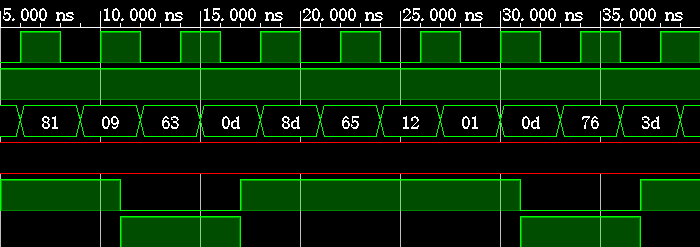
\includegraphics[width=0.8\textwidth]{1.jpg}
        \caption{FIFO1:写入的初始阶段}
    \end{figure}
    在这个波形图中, 一开始读入的是81信号, 后来是09信号, 在write\_addr=1中写入了0981
    \begin{figure}[!h]
        \centering
        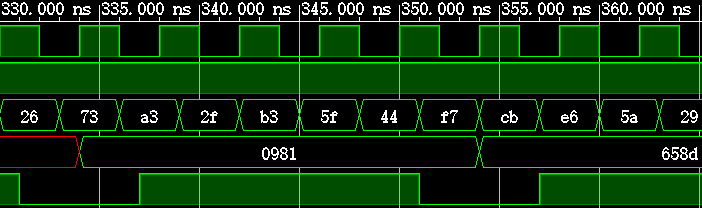
\includegraphics[width=0.8\textwidth]{2.jpg}
        \caption{FIFO1:读出的初始阶段}
    \end{figure}
    在这个波形图中输出有效, 而读出的第一个数据就是第一个写入的数据0981, 可以初步判断所设计的fifo是满足我们实验要求的
    \newpage
\subsection{FIFO:读写不影响}
    在这个实验中需要注意的是不能读出空的fifo, 所以在读出的时候需要保证read\_addr要小于write\_addr, 波形图如下
    \begin{figure}[!h]
        \centering
        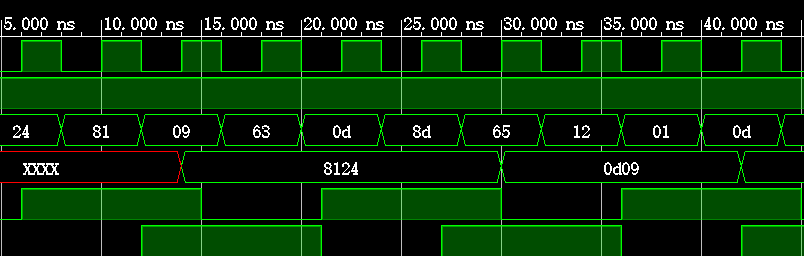
\includegraphics[width=0.8\textwidth]{3.jpg}
        \caption{FIFO2}
    \end{figure}
    可以看到, 一开始写入24,之后是81, 之后再第一个读出有效的时候读出8124, 满足实验要求
\subsection{FIFO:写入读出频率比}
    在这个实验中转化为每次写入16位,之后输出8位,调节testbench使得写入和读出的频率为2:3, 结果如下\\
    \begin{figure}[!h]
        \centering
        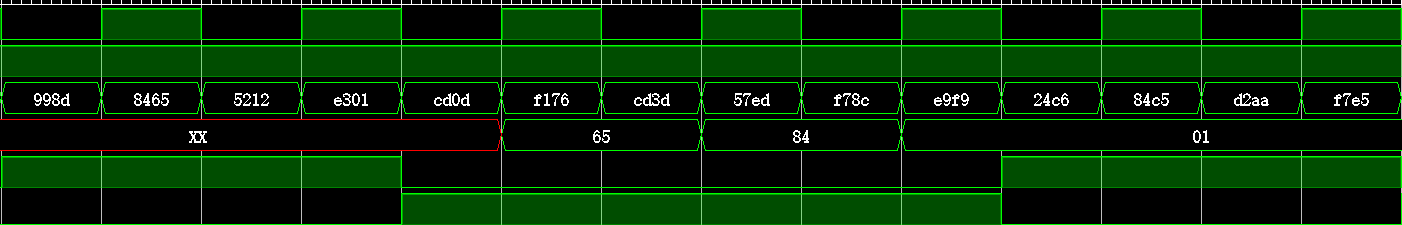
\includegraphics[width=1\textwidth]{4.jpg}
        \caption{FIFO3}
    \end{figure}\\
    一开始写入8465, 之后读出65,在读出84, 之后进入写入的阶段, 输出一直是01保持不变\\
    \begin{figure}[ht]
        \centering
        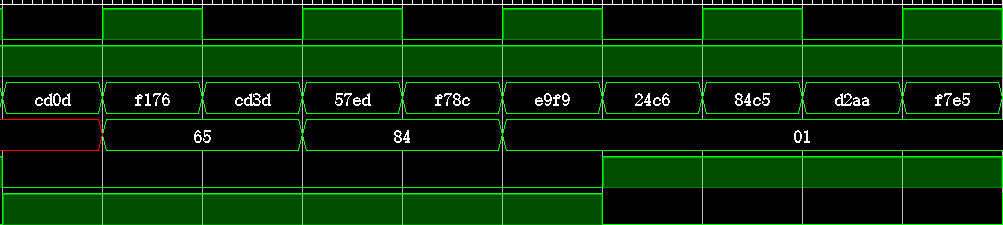
\includegraphics[width=1\textwidth]{5.jpg}
        \caption{FIFO3:分频展示}
    \end{figure}\\
    这个波形图展示了我们的写入和读出的频率为2:3, 说明我们的设计基本符合条件



\section{实验总结}
在本次实验中, 学习了fifo的原理以及设计方法, 另外值得一提的是, 我们对memory的使用也对未来有很大的帮助, 在一定程度上掌握了
有关地址索引的只是. 另外, 在本次实验中对testbench的调试占较大一部分, 对testbench的设计与调试有了更深的理解
    



\section{源代码}
    \subsection{设计文件}
    \subsubsection{FIFO1:写满才能读出}
    {\setmainfont{Courier New Bold}                               
    \begin{lstlisting}
module fifo(
    input clk,
    input rstn,
    
    input [7:0] data_in,
    input input_valid,
    
    output reg [15:0] data_out,
    input output_enable 
    //input_valid和output_enable是外部的控制信号
    );
    
    
    reg [15:0] mem [31:0];
    //表示每组数据的长度为16,一共有32组数据
    reg [6:0] write_addr;
    //表示写入时候的地址, 因为一共有32组,
    //所以在这里需要用5位来表示数据地址
    reg [6:0] read_addr;
    
    reg write;//用于表示当前fifo的状态是写入还是读出
    reg read;
    reg input_enable;
    reg output_valid;
    
    reg write_state;
    //因为是8位8位写入, 
    //所以用这样一个数据来表示写入在低8位还是高8位
    
    
    always @(negedge rstn or posedge clk)begin
        if(rstn==0)begin
            write_addr <= 6'b000000;
            //初始化读入和读出,这个保证了先入先出
            read_addr <= 6'b000000;
            input_enable <= 1;
            //表示一开始是从读入开始的
            output_valid <= 0;
            //表示一开始不读出, 只写入
            write_state <= 0;
        end
        else begin
        if(write == 1)begin//读到是写入状态
                if(write_state == 0)begin
                    write_state <= ~write_state;
                    mem[write_addr][7:0] <= data_in[7:0];
                end
                else begin
                    write_state <= ~write_state;
                    mem[write_addr][15:8] <= data_in[7:0];
                    if(write_addr < 31)begin
                    //如果是前32个广度, 继续读入
                        write_addr <= write_addr+1;
                    end
                    else begin
                    //发现地址超过31,说明写满了,转化为读出
                        input_enable <= 0;
                        output_valid <= 1;
                        write_addr <= 0;
                    end            
                end
        end
        else if(read == 1)begin
            data_out[15:0] <= mem[read_addr][15:0];
            if(read_addr < 31)begin
                read_addr <= read_addr+1;
            end
            else begin
                read_addr <= 0;
                input_enable <= 1;
                output_valid <= 0;
            end
        end
        else begin
        end
        end
    end
        
        always @(*) begin
        write = input_valid && input_enable;
        end
        
        always @(*) begin
        read = output_valid && output_enable;
        end
    
endmodule
    \end{lstlisting}}
    \subsubsection{FIFO2:读写不影响}
    {\setmainfont{Courier New Bold}                               
    \begin{lstlisting}
module fifo2(
    input clk,
    input rstn,
    
    input [7:0] data_in,
    input input_valid,
    
    output reg [15:0] data_out,
    input output_enable 
    //input_valid和output_enable是外部的控制信号
    );
    
    
    reg [15:0] mem [31:0];
    //表示每组数据的长度为16,一共有32组数据
    reg [6:0] write_addr;
    //表示写入时候的地址, 因为一共有32组,
    //所以在这里需要用5位来表示数据地址
    reg [6:0] read_addr;
    
    reg write;//用于表示当前fifo的状态是写入还是读出
    reg read;
    reg input_enable;
    reg output_valid;
    
    reg write_state;
    //因为是8位8位写入, 
    //所以用这样一个数据来表示写入在低8位还是高8位
    reg [3:0]write_period;
    reg [3:0]read_period;
    
    
    always @(negedge rstn or posedge clk)begin
        if(rstn==0)begin
            write_addr <= 6'b000000;
            //初始化读入和读出,这个保证了先入先出
            read_addr <= 6'b000000;
            input_enable <= 1;
            //表示一开始都可以读入, 读出
            output_valid <= 1;
            write_state <= 0;
            write_period <= 0;
            read_period <=0;
        end
        else begin
        if(write == 1)begin//读到是写入状态
                if(write_state == 0)begin
                    write_state <= ~write_state;
                    mem[write_addr][7:0] <= data_in[7:0];
                end
                else  begin
                    write_state <= ~write_state;
                    mem[write_addr][15:8] <= data_in[7:0];
                    if(write_addr < 31)begin//如果是前32个广度, 继续读入
                        write_addr <= write_addr+1;
                    end
                    else   begin
                    write_addr <= 0;   //后面的写满, 从头再写
                    write_period = write_period +1;//表示写完了一圈
                    end
            end
        end
        if(read == 1)begin
        //write和read并不是if-else的两端, 
        //在这种语法下二者应该可以同时进行
            if((read_addr < write_addr) || (read_period < write_period)) begin
            //用于判断接下来要读出的地址是不是没有写入数据
                data_out[15:0] = mem[read_addr][15:0];
                if(read_addr < 31) begin //检测是不是读空
                    read_addr <= read_addr+1;
                end
                else begin
                    read_addr <= 0;//表示读完了一个周期
                    read_period = read_period+1;//读的周期加1
                end
            end
            else begin//如果要读出的是空的, 就不读出
            end
        end
        end
    end

                
        always @(*) begin
        write = input_valid && input_enable;
        end
        
        always @(*) begin
        read = output_valid && output_enable;
        end
    
endmodule
    \end{lstlisting}}
    \subsubsection{FIFO3:写入读出频率比}
    {\setmainfont{Courier New Bold}                               
    \begin{lstlisting}
module fifo3(
    input clk,
    input rstn,
    
    input [15:0] data_in,
    input input_valid,
    
    output reg [7:0] data_out,
    input output_enable 
    //input_valid和output_enable是外部的控制信号
    );
    
    
    reg [15:0] mem [31:0];
    //表示每组数据的长度为16,一共有32组数据
    reg [5:0] write_addr;
    //表示写入时候的地址, 因为一共有32组,
    //所以在这里需要用5位来表示数据地址
    reg [5:0] read_addr;
    
    reg write;//用于表示当前fifo的状态是写入还是读出
    reg read;
    reg input_enable;
    reg output_valid;
    reg [3:0]write_period;
    reg [3:0]read_period;
    
    reg read_state;//因为是8位8位写入, 
    //所以用这样一个数据来表示写入在低8位还是高8位
    
    
    always @(negedge rstn or posedge clk)begin
        if(rstn==0)begin
            write_addr <= 5'b000000;
            //初始化读入和读出,这个保证了先入先出
            read_addr <= 5'b000000;
            input_enable <= 1;
            //表示一开始都可以读入, 读出
            output_valid <= 1;
            read_state <= 0;
            read_period <= 0;
            write_period <= 0;
        end
        else begin
        if(write == 1)begin//读到是写入状态
            mem[write_addr][15:0] <= data_in[15:0];
            //每次写入16位数据
                    if(write_addr < 31)begin
                    //如果是前32个广度, 继续读入
                        write_addr <= write_addr+1;
                    end
                    else   begin
                    write_addr <= 0;
                    write_period = write_period + 1;    
                    //如果已经写满了,就不能继续写了    
                    end
            end
        end
        if(read == 1)begin
        //write和read并不是if-else的两端, 
        //在这种语法下二者应该可以同时进行
            if(read_addr < write_addr || read_period < write_period) begin
            //用于判断接下来要读出的地址是不是没有写入数据
                if(read_state == 0) begin
                    read_state <= ~read_state;
                    data_out[7:0] <= mem[read_addr][7:0];
                end
                else begin
                    read_state <= ~read_state;
                    data_out[7:0] <= mem[read_addr][15:8];
                    if(read_addr < 31)begin
                        read_addr <= read_addr+1;
                    end
                    else begin
                    read_addr <= 0;
                    read_period = read_period+1;
                    end
                end
            end
            else begin//如果要读出的是空的, 就不读出
            end
        end
        end
        
        always @(*) begin
        write = input_valid && input_enable;
        end
        
        always @(*) begin
        read = output_valid && output_enable;
        end
        
endmodule
    \end{lstlisting}}


       
\subsection{激励文件}
\subsubsection{FIFO1:写满才能读出}
{\setmainfont{Courier New Bold}                               
\begin{lstlisting}
module test_sim_fifo(

    );
    
    reg clk,rstn;
    reg [7:0] data;
    wire [15:0] out;
    reg input_valid, output_enable;
    
    fifo test_sim_fifo(
        .clk(clk),
        .rstn(rstn),
        .input_valid(input_valid),
        .output_enable(output_enable),
        .data_in(data),
        .data_out(out)
     );
     
     always #2 begin
        clk = ~clk;
        end
    
     initial begin
        clk = 1'b0;
        rstn = 1'b1;
        input_valid = 1'b0;
        output_enable = 1'b0;
        #1 rstn = 1'b0;
        #2 rstn = 1'b1;
     end
     
     always begin
        #3;
        data = $random()%9'b1_0000_0000;    //输入是8位
     end
     
     always begin
        #5;
        input_valid = 1'b1;
        #6;
        input_valid = 1'b0;
        output_enable = 1'b1;
        #6;
        input_valid = 1'b1;
        output_enable = 1'b0;
        #3;

     end
endmodule
\end{lstlisting}}
\subsubsection{FIFO2:读写不影响}
{\setmainfont{Courier New Bold}                               
\begin{lstlisting}
module test_fifo2(

);
    
    reg clk,rstn;
    reg [7:0] data;
    wire [15:0] out;
    reg input_valid, output_enable;
    
    fifo2 test_sim_fifo(
        .clk(clk),
        .rstn(rstn),
        .input_valid(input_valid),
        .output_enable(output_enable),
        .data_in(data),
        .data_out(out)
     );
     
     always #2 begin
        clk = ~clk;
        end
    
     initial begin
        clk = 1'b0;
        rstn = 1'b1;
        input_valid = 1'b0;
        output_enable = 1'b0;
        #1 rstn = 1'b0;
        #2 rstn = 1'b1;
     end
     
     always begin
        #4;
        data = $random()%9'b1_0000_0000;    //输入是8位
     end
     
     always begin
        #6;
        input_valid = 1'b1;
        output_enable = 1'b0;
        #6;
        input_valid = 1'b1;
        output_enable = 1'b1;
        #3;
        input_valid = 1'b0;
        output_enable = 1'b1;
        //$finish;
     end
endmodule
\end{lstlisting}}
\subsubsection{FIFO3:写入读出频率比}
{\setmainfont{Courier New Bold}                               
\begin{lstlisting}
module test_fifo3(

    );
    
    reg clk,rstn;
    reg [15:0] data;
    wire [7:0] out;
    reg input_valid, output_enable;
    
    fifo3 test_sim_fifo(
        .clk(clk),
        .rstn(rstn),
        .input_valid(input_valid),
        .output_enable(output_enable),
        .data_in(data),
        .data_out(out)
     );
     
     always #2 begin
        clk = ~clk;
        end
    
     initial begin
        clk = 1'b0;
        rstn = 1'b1;
        input_valid = 1'b0;
        output_enable = 1'b0;
        #1 rstn = 1'b0;
        #2 rstn = 1'b1;
     end
     
     always begin
        #2;
        data = $random()%17'b1_0000_0000_0000_0000;    //输入是8位
     end
     
     always begin
        #12;
        input_valid = 1'b1;
        output_enable = 1'b0;
        #8;
        input_valid = 1'b0;
        output_enable = 1'b1;
     end
endmodule
\end{lstlisting}}


\end{document}